\documentclass[10pt, twocolumn]{article}

%----------------------------------------------
%-----------------Packages---------------------
%----------------------------------------------

% Writing 
\usepackage[english]{babel}
\usepackage[utf8]{inputenc}
\usepackage[pdftex]{lscape}
\fontfamily{times}
\usepackage[affil-it]{authblk}
\usepackage{lettrine}

% Graphics
\usepackage{caption}
\usepackage{float}
\usepackage{subcaption}
\usepackage{graphicx}
\usepackage[outdir=./images/]{epstopdf}
\graphicspath{{images/}}

% Math
\usepackage{amsthm, amssymb, amsmath, mathtools}

% Biblio
\usepackage[numbers]{natbib}
\bibliographystyle{apalike}

%Others
\usepackage{xurl}
\PassOptionsToPackage{hyphens}{url}
\usepackage[colorlinks=true,citecolor=blue,linkcolor=magenta]{hyperref}
\usepackage{ifthen}
\usepackage{multirow}
\usepackage{lipsum}


%----------------------------------------------
%---------------Math definitions---------------
%----------------------------------------------

\newcommand{\R}{\mathbb{R}}
\newcommand{\bb}[1]{\boldsymbol{#1}}


%----------------------------------------------
%--------------Other definitions---------------
%----------------------------------------------

\newcommand{\com}[1]{\textcolor{red}{#1}}
\newcommand{\BL}[1]{\lettrine{\textbf{#1}}{}}


%----------------------------------------------
%-----------------Title Page-------------------
%----------------------------------------------

\title{Air pollution forecasting in Rio de Janeiro
        \vspace{2mm}
       \\\large Final assignment on the subject Machine Learning 
}

\author{Lucas Machado Moschen}
\affil{School of Applied Mathematics, \\ Fundação Getulio Vargas}

\date{\today}

%----------------------------------------------
%------------------Document--------------------
%----------------------------------------------


\begin{document}

\newcounter{num}
\setcounter{num}{0}

\twocolumn[
    \begin{@twocolumnfalse}

        \maketitle

        \begin{abstract}
            Air is an essential resource and its quality is important for the human being
and the environment. The ability to understand and predict air quality may
help to prevent events of poor quality and formulate environmental policies.
This work presents models for O$_3$, CO, and PM$_{10}$ for each monitoring
station in Rio de Janeiro. Machine learning methods, including linear
regression, support vector machine, and random forest produced promising
results for gases and AQI levels predictions. 

\vspace{6mm}
        \end{abstract}

        \vspace{7mm}

    \end{@twocolumnfalse}
]

\section{Introduction}

\lettrine[findent=2pt]{\textbf{R}}{}io de Janeiro city (Brazil) is one of the
most beautiful cities in the world, according to the travel website Conde Nast
Traveler \cite{travelRio}. This thought is shared among tourists and
residents.

\begin{enumerate}
    \item What is the problem? 
    \item Why is it important? 
    \item What is your basic approach? 
    \item A short discussion of how it fits into related work in the area is also desirable.
    \item Basic results. 
    \item Conclusions
\end{enumerate}

\section{Problem definition}

\begin{enumerate}
    \item What is the problem?
    \item What are the inputs and outputs mathematically. 
\end{enumerate}
\section{Background of air pollution}

Air pollution is a mixture of particles and gases, often not visible to human
eyes. The visible forms are widely known, such as smoke, soot and mold.
\com{The quality air index, calculated based on the levels of the gases, is
available in a diary report}, as presented in image XXX.  

\subsection{Polluting gases}

The atmosphere of the Earth is a dynamic and complex system of natural gases,
which are necessary to life, according to \cite{gases}. The planet has a
defense mechanism that absorbs part of these fases, what forms a cycle.
However, high levels of gases concentration can cause several effects in the
living beings. The polluting gases include: 

\begin{itemize}
    \item \textbf{Óxidos de Carbono:} O monóxido de carbono (CO) é oriundo da
    combustão incompleta e não apresenta cheiro ou cor. Já o dióxido de
    carbono é um gás que contribui para o efeito estufa e, em excesso na
    atmosfera, devido à queima de combustíveis fósseis, pode causas sérios
    danos.  
    \item \textbf{Óxidos de Nitrogênio:} Também emitidos por veículos e
    tem uma aparência marrom. O dióxido de nitrogênio é um dos gases mais
    perigosos para a poluição do ar, e sua toxidade é facilmente
    identificável. 
    \item \textbf{Óxidos de Enxofre:} Causa primária da chuva ácida, muito
    comum na Europa. É natural após erupções vulcânicas. É uma forte causa de
    problemas respiratórios. 
    \item \textbf{Ozônio:} O gás ozônio ($O_3$) contém três átomos de oxigênio. Até pequenas
    concentrações desse gás são consideradas tóxicas e explosivas. Ele ocorre
    naturalmente na atmosfera, porém em pequenas quantidades, quando absorve
    radiação ultravioleta. Em condições especiais, óxidos de nitrogênio e
    hidrocarbonos podem produzir ozônio em concentração alta o suficiente para
    causar irritação nos olhos e na mucosa. 
\end{itemize}



\section{Methodology}
\label{sec:methodology}

\BL{E}xploratory data analysis is the first step into the project, after
identifying the problem. The proposed EDA includes visualization and descriptive statistics to
summarize the most relevant information to have insights. After this, we make
data preprocessing, which includes missing data imputation, outlies, and
feature engineering.   

The evaluation methods for the algorithms are the mean absolute error (MAE), the root
mean squared error (RMSE), and the normalized RMSE (nRMSE). The methods were
trained using 70\% of the available data, considering the first years. The
software used for performing this experimental phase was developed in Python (version 3.9), mainly using the Pandas and Scikit-learn.

\section{Exploratory data analysis}
\label{sec:eda}

\subsection{Data description}

\BL{T}he dataset used in this study was extracted from the project MonitorAr-Rio
\cite{dataset-rio-ar-quality}. The table contains hourly data observations, separated by
pollutant, weather condition, and monitoring stations' characteristics from
the city of Rio de Janeiro. Table
\ref{tab:measured-data} informs the most important variables used, and Table
\ref{tab:pollutants-measured} indicates the measured pollutants per monitoring
station. The events start on January 1,
2011,
and end on March 31, 2021, totalizing 661,662 records.

The missing values (Table \ref{tab:missing-values}) for each of the main variables used in this work 
are around 10\%. Some meteorological variables have more than 10\% of missing values, which is a lot.
The CO gas has more missing values than the other gases because Pedra de
Guaratiba does not measure it. When this kind of absent value is disregarded,
CO has around 6\%. Imputation methods in Section \ref{sec:data-preprocessing}.

Almost 91\% of the values in {\tt Chuva} column and 26\% in {\tt RS} column are zero. If we consider the accumulated monthly amount of
rain, it seems to make sense, and it is comparable to other sources. 

We did not observe any pattern of missing values per year or monitoring
station. In 2012, over half of the wind information is missing, however other
features are stable. After 2016, UR dominates the number of absent
data. If we aggregate by time (hour, day, month, and year), and sum up the
values of the features of each station, there are less missing data,
proportionally. This
implies that other stations can provide useful information. 

\begin{table*}[t]
    \centering
    \begin{tabular}{c|c|c|c|}
        \cline{2-4}
       & \textbf{Name} & \textbf{Type} & \textbf{Description}              \\ \hline
        \multicolumn{1}{|c|}{\multirow{7}{*}{\textbf{meteorological conditions}}} & Chuva         & float         & Rainfall (mm)                     \\ \cline{2-4} 
        \multicolumn{1}{|c|}{}                                                   & Pres          & float         & Atmospheric Pressure (mbar)       \\ \cline{2-4} 
        \multicolumn{1}{|c|}{}                                                   & RS            & float         & Solar radiation (w/m2)            \\ \cline{2-4} 
        \multicolumn{1}{|c|}{}                                                   & Temp          & float         & Temperature (°C)                  \\ \cline{2-4} 
        \multicolumn{1}{|c|}{}                                                   & UR            & float         & Relative humidity (\%)            \\ \cline{2-4} 
        \multicolumn{1}{|c|}{}                                                   & Dir\_Vento    & float         & Wind direction (°)                \\ \cline{2-4} 
        \multicolumn{1}{|c|}{}                                                   & Vel\_Vento    & float         & Wind speed (m/s)                  \\ \hline
        \multicolumn{1}{|c|}{\multirow{5}{*}{\textbf{Measurement conditions}}}   & Data          & datetime      & Measurement date and hour         \\ \cline{2-4} 
        \multicolumn{1}{|c|}{}                                                   & CodNum        & integer        & Number of the monitoring station  \\ \cline{2-4} 
        \multicolumn{1}{|c|}{}                                                   & Estação       & string        & Name of the monitoring station    \\ \cline{2-4} 
        \multicolumn{1}{|c|}{}                                                   & Lat           & float         & Latitude position of the station  \\ \cline{2-4} 
        \multicolumn{1}{|c|}{}                                                   & Lon           & float         & Longitude position of the station \\ \hline
        \end{tabular}
    \caption{Measured parameters by the program MonitorAr.}
    \label{tab:measured-data}
\end{table*}

\begin{table*}[t]
    \centering
    \begin{tabular}{|c|c|}
    \hline
    \textbf{Monitoring station}        & \textbf{Measured gases/particulates}              \\ \hline
    Centro (CA)             & O$_3$, CO, PM$_{10}$                              \\ \hline
    Copacabana (AV)         & SO$_2$, O$_3$, CO, PM$_{10}$                      \\ \hline
    São Cristóvão (SC)      & SO$_2$, O$_3$, CO, PM$_{10}$                      \\ \hline
    Tijuca (SP)             & SO$_2$, NOx, O$_3$, CO, PM$_{10}$                 \\ \hline
    Irajá (IR)              & SO$_2$, NOx, O$_3$, CO, HC, PM$_{2.5}$, PM$_{10}$ \\ \hline
    Bangu (BG)              & SO$_2$, NOx, O$_3$, CO, HC, PM$_{10}$             \\ \hline
    Campo Grande (CG)       & SO$_2$, NOx, O$_3$, CO, HC, PM$_{10}$             \\ \hline
    Pedra de Guaratiba (PG) & O$_3$, PM$_{10}$                                  \\ \hline
    \end{tabular}
    \caption{Pollutant data measured by each monitoring station. CO and HC are measured in (ppm), while the others are measured in (µg/m3).}
    \label{tab:pollutants-measured}
\end{table*}

\begin{figure*}[ht]
    \centering
    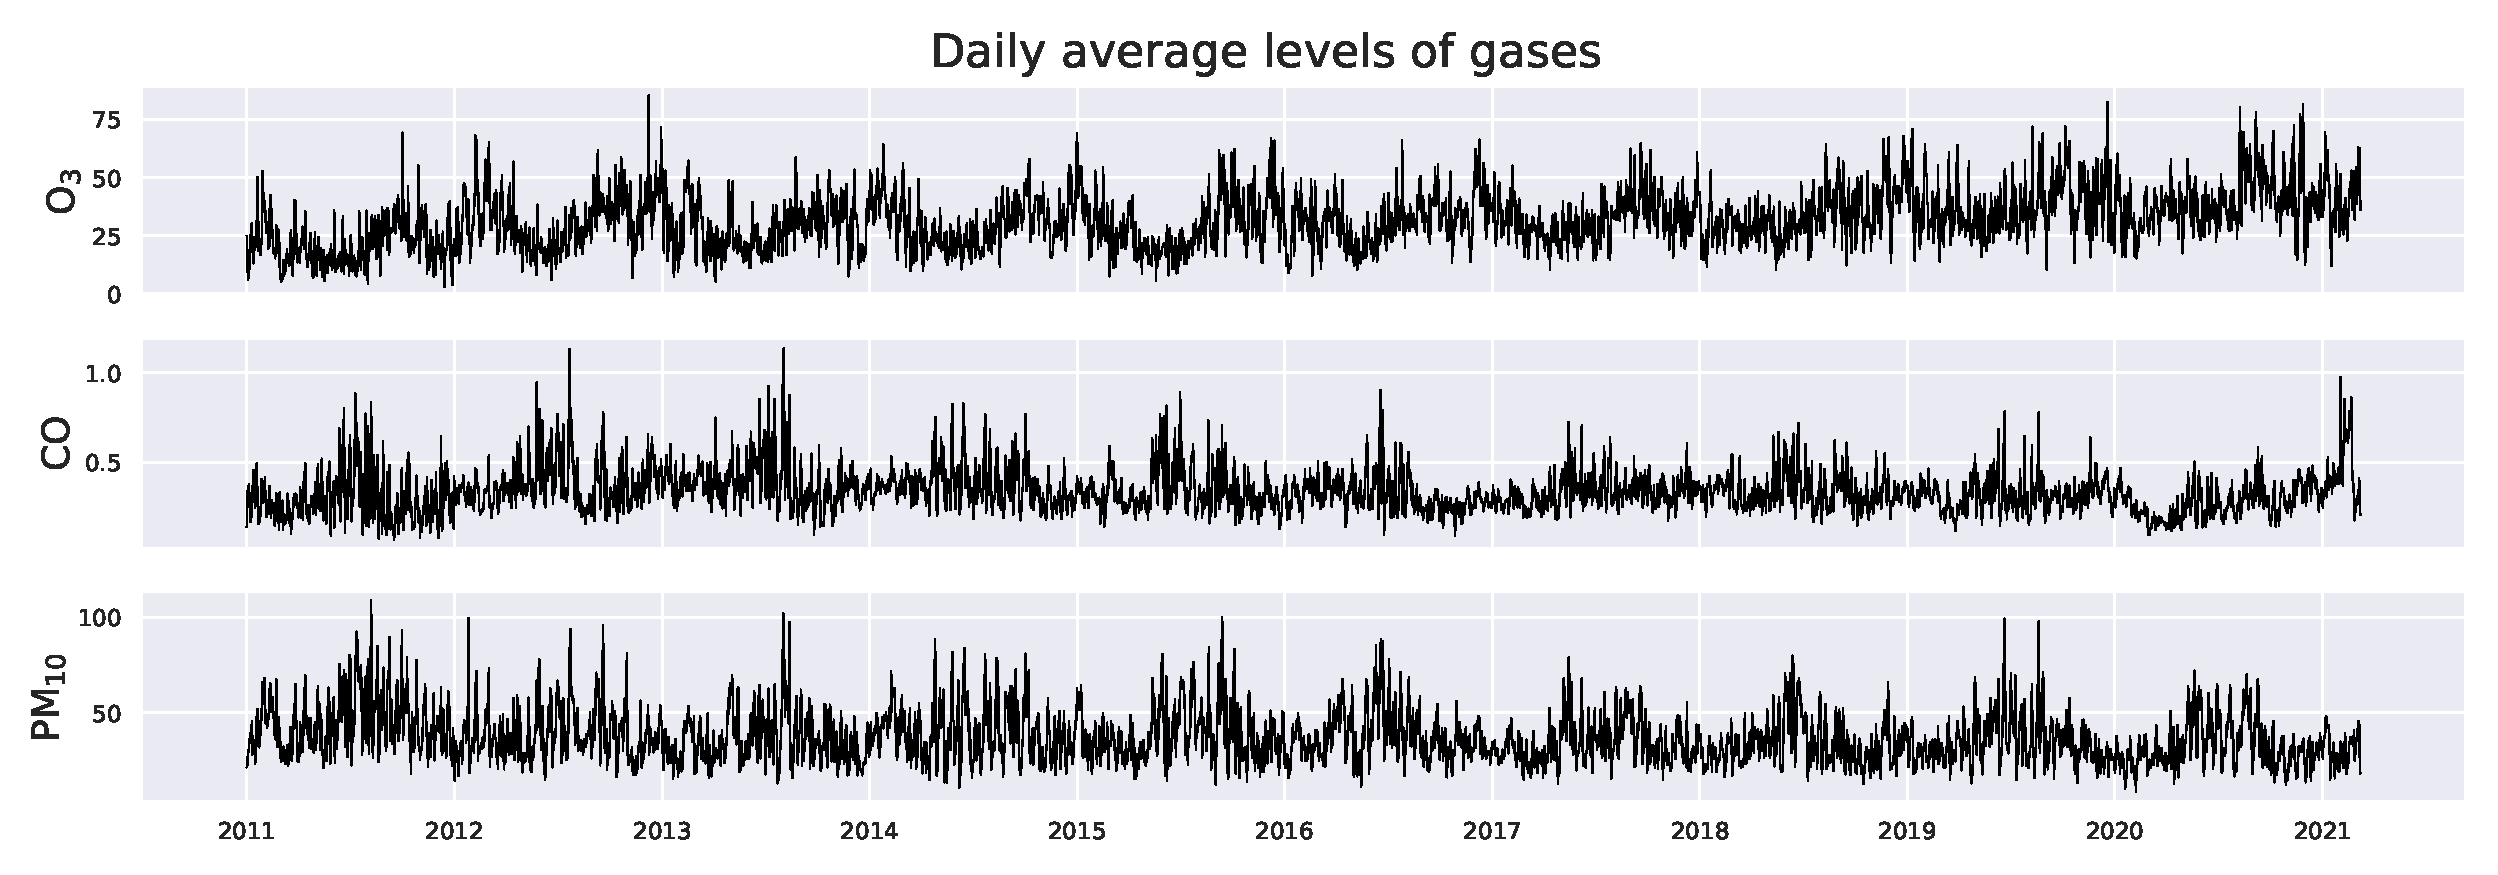
\includegraphics[width=\textwidth]{time-plots-gases.eps}
    \caption{Time series with diary average levels.}
    \label{fig:time-series-gases}
\end{figure*}

\begin{table}
    \centering
    \begin{tabular}{|c|c|}
        \hline
        {\bf Variable} & {\bf Missing values} \\\hline
        Chuva     &   15812 (2.38 \%) \\\hline
        Pres      &   15294 (2.31 \%) \\\hline
        RS        &   48260 (7.29 \%) \\\hline
        Temp      &   70617 (10.6 \%) \\\hline
        UR        &  110619 (16.7 \%) \\\hline
        Dir\_Vento &   90498 (13.6 \%) \\\hline
        Vel\_Vento &   90743 (13.7 \%) \\\hline
        CO        &  114179 (17.2 \%) \\\hline
        O3        &   37133 (5.61 \%) \\\hline
        PM10      &   36142 (5.46 \%) \\\hline
    \end{tabular}
    \caption{Missing data in absolute and proportional values of the main variables. Data, CodNum, Lat, and Lon do not have nan values.}
    \label{tab:missing-values}    
\end{table}

Table \ref{tab:statistics-variables} contains the summary statistics of the variables. The high skewness and kurtosis from {\tt
Chuva} column reaffirm the heavy tails of its distribution, or the presence of
outliers. The same occurs with {\tt Press}. This is interesting because, it is common to see days with
extreme values in meteorological variables. In particular, the only hours with
precipitation greater than 100 mm were in May 2020 in Tijuca, what is
confirmed by weather references \cite{climatempo}. CO and PM$_{10}$ have high
kurtosis also and, therefore, can have outliers. 

\begin{table*}[t]
    \centering
    \begin{tabular}{|c|c|c|c|c|c|c|c|c|c|c|}
        \hline
        {} & {\bf Chuva} &  {\bf Pres} & {\bf RS} & {\bf Temp} & {\bf UR} &
        {\bf Dir} & {\bf Vel} & {\bf CO} & {\bf O3} & {\bf PM10} \\
        \hline
        {\bf Mean}  &       0.13 &    1014.65 &     152.82 &      26.12 &      70.90
        &     163.73 &       1.21 &       0.34 &      31.98 &      36.91 \\
        \hline
        {\bf Std}   &       1.64 &       5.68 &     244.37 &       4.90 &      18.35
        &      73.45 &       1.00 &       0.28 &      29.81 &      23.52 \\
        \hline
        {\bf Min}   &       0.00 &     800.00 &       0.00 &       0.00 &       0.00
        &       0.00 &       0.00 &       0.00 &       0.00 &       0.00 \\
        \hline
        {\bf 25\%}   &       0.00 &    1011.12 &       0.00 &      22.67 &
        58.39 &     100.00 &       0.55 &       0.14 &       8.68 &      21.00
        \\
        \hline
        {\bf 50\%}   &       0.00 &    1014.30 &       6.17 &      25.54 &
        72.75 &     166.17 &       0.92 &       0.29 &      24.52 &      32.00
        \\
        \hline
        {\bf 75\%}   &       0.00 &    1018.02 &     224.00 &      28.99 &
        85.08 &     222.50 &       1.55 &       0.46 &      46.89 &      47.00
        \\
        \hline
        {\bf Max}   &     426.60 &    1036.48 &    1864.67 &      49.08 &     100.00
        &     358.83 &      25.50 &      12.08 &     355.45 &     994.00 \\
        \hline
        {\bf Skew}  &     114.55 &      -7.32 &       1.61 &       0.55 &      -0.44
        &       0.04 &       3.74 &       2.75 &       1.56 &       2.72 \\
        \hline
        {\bf Kurt}  &   23177.40 &     282.90 &       1.48 &       0.33 &      -0.40
        &      -0.97 &      47.30 &      24.85 &       3.71 &      38.67 \\
        \hline
    \end{tabular}
    \caption{Statistics of the meteorological variables and gases.}
    \label{tab:statistics-variables}
\end{table*}


The time series of the three gases are presented in Figure
\ref{fig:time-series-gases}. It indicates growth in ozone levels during the
years and a seasonal effect, which corroborates the way ozone is formed.  It
also seems there is a decrease in variability in CO and PM$_{10}$ levels. The
year 2020 shows a reduction in CO apparently, which is explained by the
Coronavirus pandemic. 

We confirm the tendencies of PM$_{10}$ and O$_3$ in Figure \ref{fig:time-series-gases-year}. It is important to note that
2021 is not finished, so seasonal effects are not complete yet.

\begin{figure}[!ht]
    \centering
    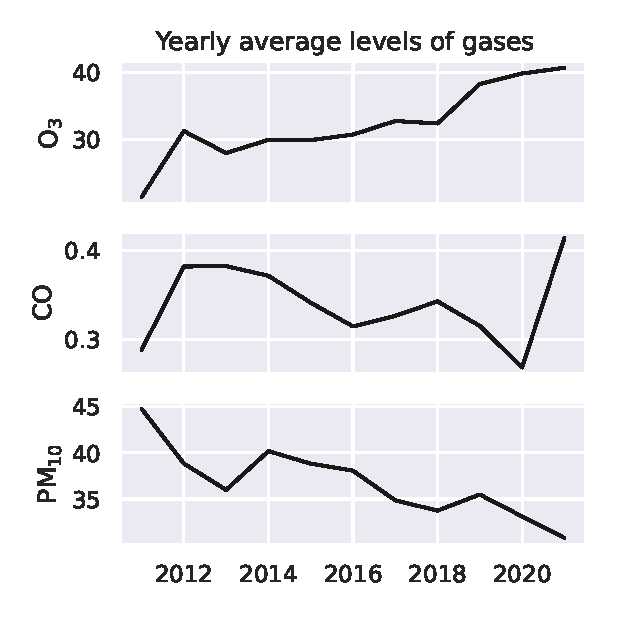
\includegraphics[width=.45\textwidth]{time-plots-gases-yearly.eps}
    \caption{Time series with yearly average levels.}
    \label{fig:time-series-gases-year}
\end{figure}

By Figure \ref{fig:histogram-obs-years}, years 2011 and 2021 have less
observations than the others. The year 2021 did not end as previously
mentioned and the year 2011 had less monitoring stations.  

\begin{figure}
    \begin{center}
        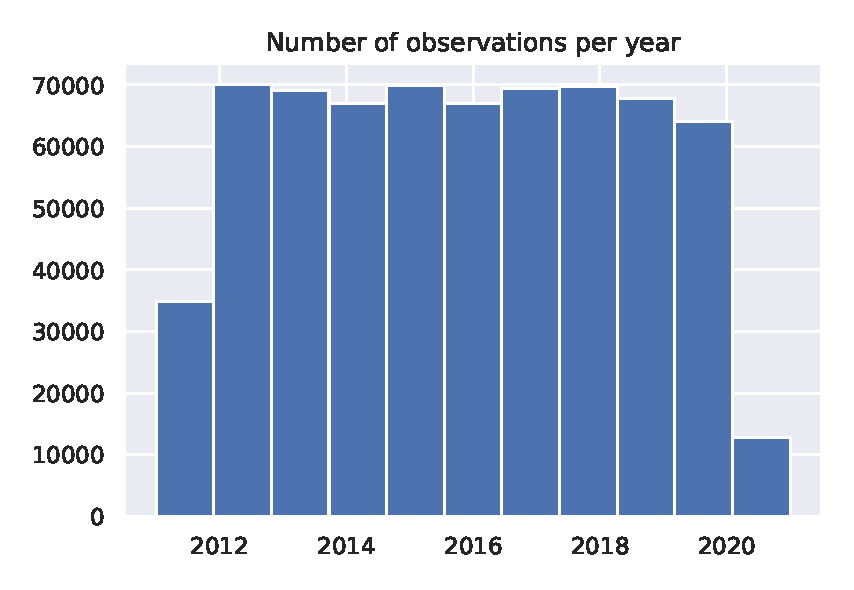
\includegraphics[width=0.47\textwidth]{histogram.eps}
    \end{center}
    \caption{Number of hourly measurements per year. In 2011, only half of the monitoring stations worked.}
    \label{fig:histogram-obs-years}
\end{figure}

Figure \ref{fig:correlation-features} shows an overview of the correlations
between different features of the data to identify possible linear relations.
The scatter plots of two to two features represents it with more details, but
there is much data, and the image has a large size. It does not present anything
much different, though. The variables {\tt Temp}, {\tt UR}, and {\tt RS} are
strongly linearly related with absolute correlation greater than 0.6.

\begin{figure*}[t]
    \begin{center}
        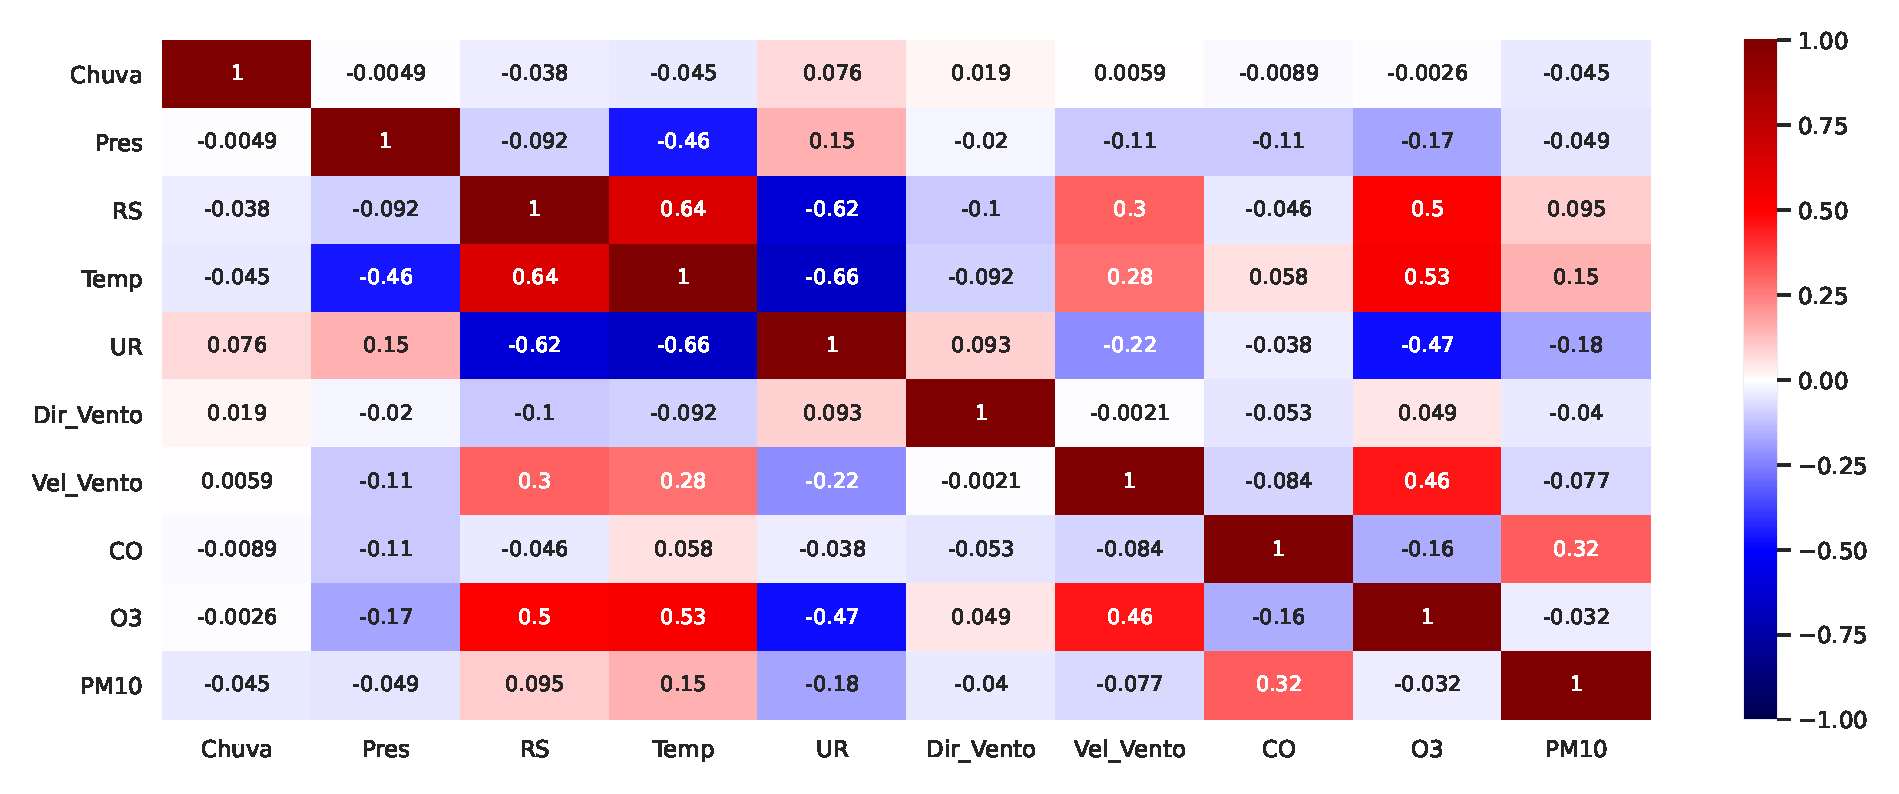
\includegraphics[width=0.9\textwidth]{correlation-graph.eps}
    \end{center}
    \caption{Correlation heat map comparing the data features.}
    \label{fig:correlation-features}
\end{figure*}

Figure \ref{fig:hourly-boxplot-ozone} shows an interesting behavior of ozone during the day. For each hour of the day, we represent the distribution of ozone in the respective hour. We
observe that (1) the pollutants have heavy tail, or this data has a lot of
outliers; and (2) the medians go along with the movement of the sun.

\vspace{-0.5cm}

\begin{figure}[H]
    \begin{center}
        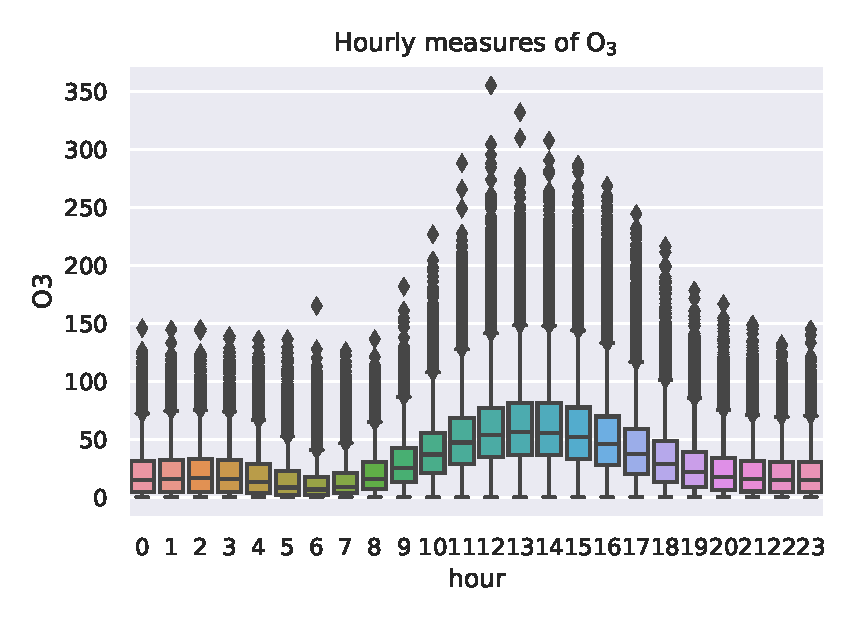
\includegraphics[width=0.42\textwidth]{hourly_measure_o3.eps}
    \end{center}
    \vspace{-0.8cm}
    \caption{Boxplot of hourly ozone measurements. }
    \label{fig:hourly-boxplot-ozone}
\end{figure}


\subsection{Data preprocessing}
\label{sec:data-preprocessing}

The data preprocessing is an essencial step before the usage of machine
learning algorithms, in order to report robust and neat results. Data from
year 2020 and 2021 will be removed given the pandemic in the world. 

\subsubsection{Seasonal and time features}

From variable {\tt Data}, it is extracted the variables {\tt year, month,
day}, {\tt hour}, a boolean variable indicating the weekend, and a {\tt season} variable. In
order to consider the hourly seasonality, it is created the variables
$\text{hour\_sin} = \sin(2\pi \text{ hour}/24)$ and $\text{hour\_cos} =
\cos(2\pi \text{ hour}/24)$. 

\subsubsection{Missing data imputation}

In this dataset, there is two types of missing data: (1) monitoring stations
do not measure all pollutants by construction. For instance, it is not
measured CO in Pedra de Guaratiba; and (2) monitoring stations did not
measure in a period for some reason. For the first case, missing values remain
in the dataset and the prediction is not performed. For the second case, three
methods were compared:  

\begin{enumerate}
    \item {\bf Simple mean imputation:} For each year and each column, the
    algorithm imputes the mean in the NaN values. 
    \item {\bf Location:} For each time period, the missing values are
    replaced by the average among the others measuring stations. For example, if
    CO is missing at 6h on 01/01/2011 at Centro station, it is replaced by the
    mean among the other stations in the same time. 
    \item {\bf k-NN:} For each year, if a feature is missing in row $i$, the
    algorithm selects the $k$ closer points according to the nan euclidean
    measure. This measure calculates the euclidean distance among non NaN
    entries and rescale depending on the number of them. The years are
    separated to reduce the number of rows.
\end{enumerate}

The data values are normalized to the range of $[0,1]$, because k-NN is based
on a distance measure. To evaluate these methods, we develop a sample strategy
similar to the Bootstrap method. In each simulation, we sample 20\% of rows with
non NaN values and randomly choose 7\% of the cells to be removed (this value
was chosen because this was observed across the entire dataset). From the simulated
dataset with missing values, the methods impute as explained before. We
compare the imputed sample after imputation with the sample before removal and calculate
the mean squared error. The results for the year 2016 are in Table \ref{tab:result-imputation}. 

\begin{table}[!hb]
    \centering
    \begin{tabular}{|c|c|}
    \hline
    \textbf{Método}   & \textbf{MSE} \\ \hline
    5-NN              & 6.504e-04    \\ \hline
    10-NN             & 6.504e-04    \\ \hline
    30-NN             & 6.504e-04    \\ \hline
    50-NN             & 6.504e-04    \\ \hline
    100-NN            & 6.504e-04    \\ \hline
    Location          & 1.077e-03    \\ \hline
    Simple Imputation & 1.636e-03    \\ \hline
    \end{tabular}
    \caption{Results from the imputation}
    \label{tab:result-imputation}
\end{table}

For that reason, we apply the 5-NN in the dataset per year to impute data. It
is important to note that the computation was a real barrier for a more deep
analysis. 

\subsubsection{Data transformation}
\label{sec:data-transform}

We applied the Yeo-Johnson power transform \cite{yeo2000} on continuous
variables in order to approximate the data distribution to a Gaussian
distribution and to
decrease the heteroscedasticity, as suggested by \cite{gocheva2014}. In figure
\ref{fig:before-after-transform}, the gases distribution (disregarded
missing data imputation) are shown before and after the transformation. The
selected $\lambda$ for each feature was estimated through maximum likelihood.
Following the order from table \ref{tab:statistics-variables}, the values
were, approximately,  
-20.16, 12.58, -0.1, 0.29, 1.59, 0.81, -0.79, -1.69, 0.28, and 0.27.

\begin{figure*}
    \centering
    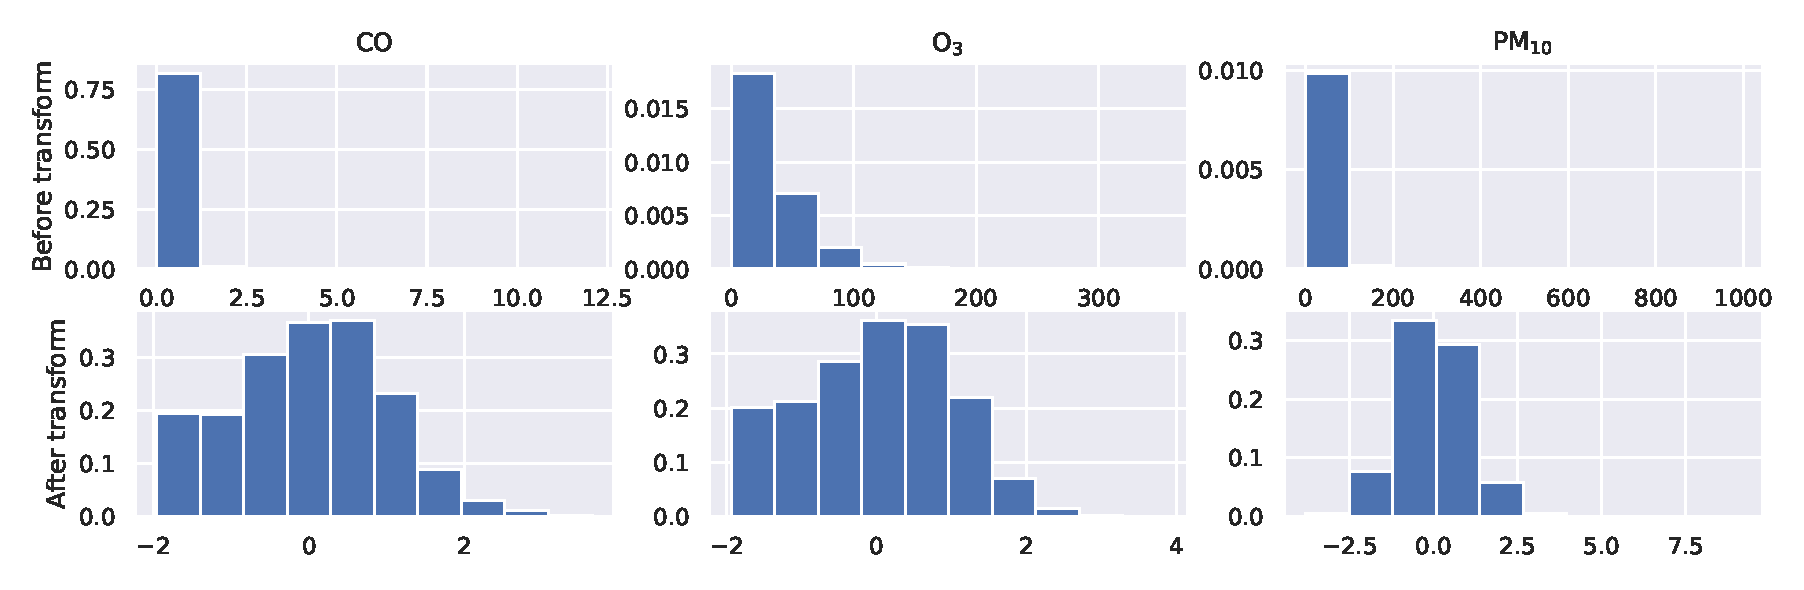
\includegraphics[width = 0.9\textwidth]{before_after_transform_gases.eps}
    \caption{Gases distribution before and after the power transform.}
    \label{fig:before-after-transform}
\end{figure*}
 
\subsubsection{Feature extraction}

The lag is a time gap in the series and are useful to analyse seasonality and trend. In
general, besides the influence of another variables, the past values can be
helpful to make good predictions. An exploratory study with autocorrelation
(ACF) and partial autocorrelation (PACF) to define the number of lag
variables. Figure \ref{fig:acf-pacf} shows interesting patterns: CO has spikes
at 12 multiples. That indicates a high correlation with twelve hours
difference. The ozone does not have this quality, but presents the diary
spikes. It is interesting that at Bangu station, this is negatively related.
Since the PACF has only two spikes in all graphs, there is an autoregressive
term in the pollutants series of order two. We add two lag variables for each
pollutant and each monitoring station, then. We also add a 24 lag time to
catch the diary influence. Besides that, a rolling mean variable with a 24 lag
is added to simulate a moving average (MA) term. It is not possible to use the MA
model in this framework since they are not observed \cite{liang2020machine}. 

\begin{figure*}
    \centering
    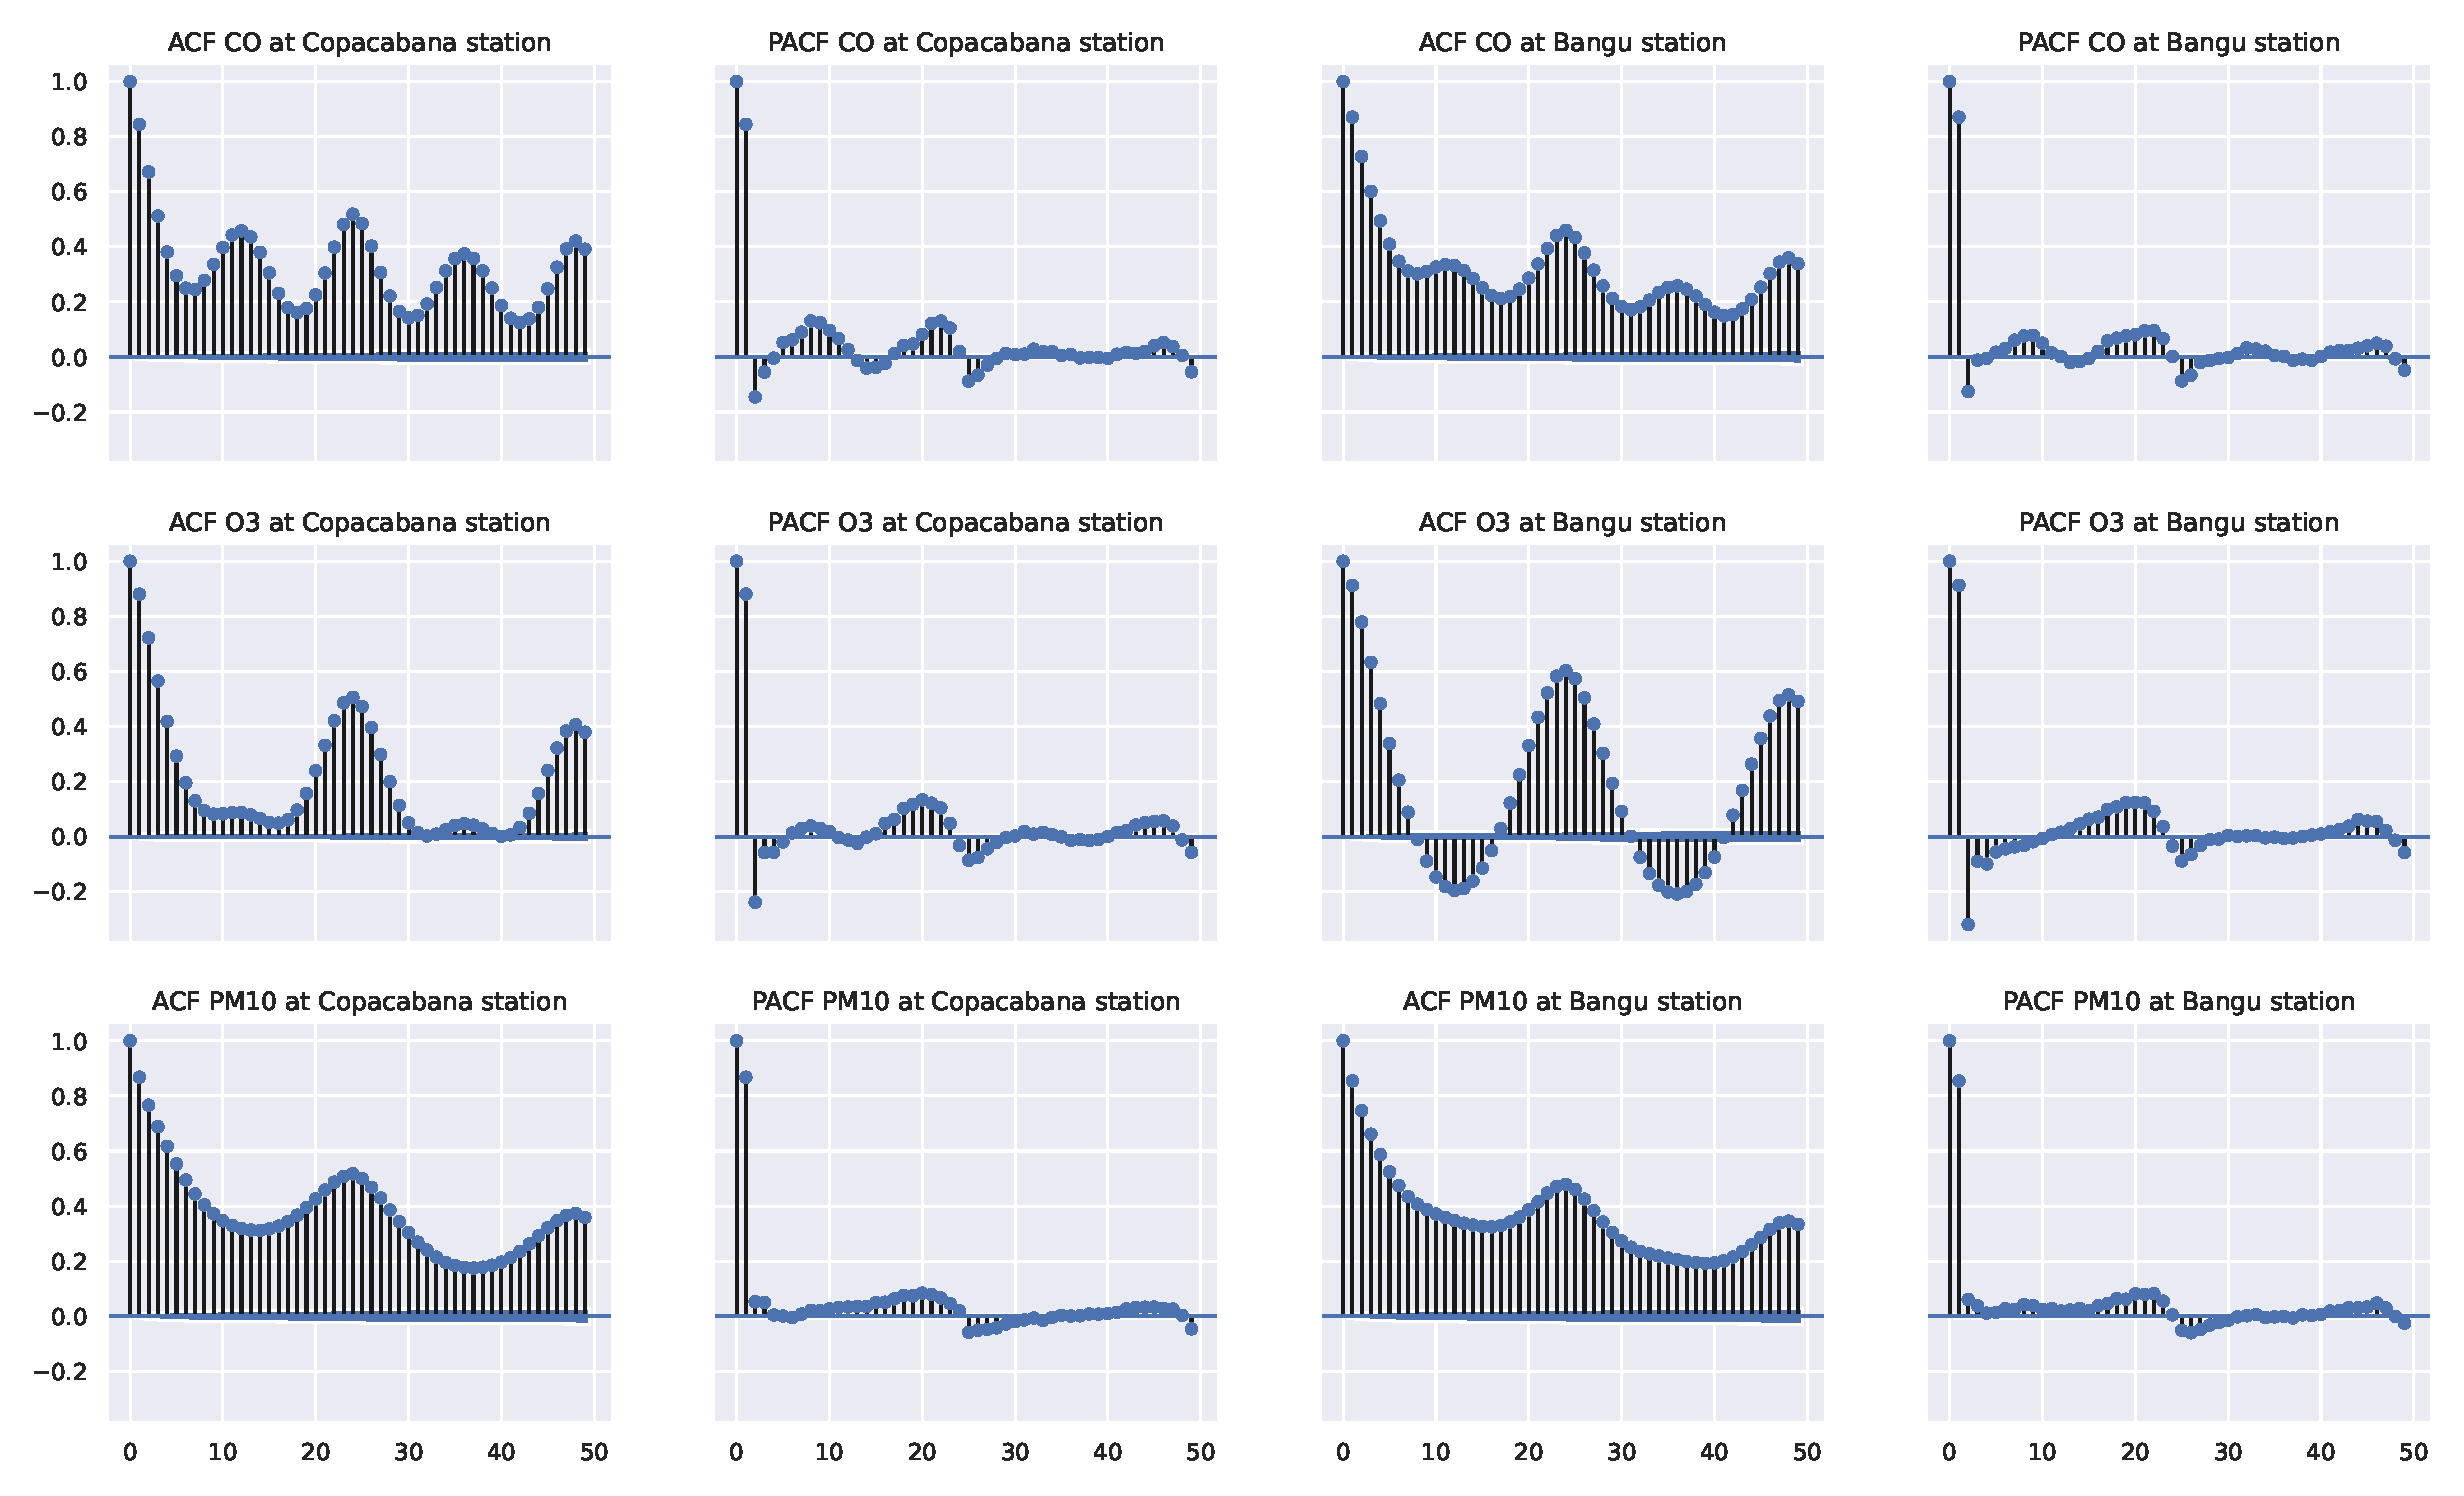
\includegraphics[width = 0.9\textwidth]{acf_pacf_gases.eps}
    \caption{ACF and PACF plots for CO, O$_3$, and PM$_{10}$ at Copacabana and
    Bangu stations. }
    \label{fig:acf-pacf}
\end{figure*}

Variables to remove: {\tt hour} since it is highly correlated with {\tt hour\_sin}, and {\tt Data}, because it has no service anymore. We will have
only numeric variables from now on. The total number of features after all
the above processes is 32 including meteorological conditions, time-related,
lags, moving averages, 
and pollutants measurements.

\begin{remark}
    The first 5 variables in PCA decomposition had more than 0.9 of explained
    variance. However, their $R^2$ score in Linear Regression was 0.616, much
    lower than the Linear Regression case explained posteriorly. For that
    reason, we ignore the reduced dataset by PCA.  
\end{remark}
\section{Experiment settings}
\label{sec:experiments}

We have already separated the dataset into training and testing. In this
section we describe the methods used for the estimation: {\em Linear
Regression}, {\em Support Vector Machine}, {\em Random Forest}, {\em
Boosting}, and a model that handle missing data simultaneously with the
fitting, using the {\em Expectation Maximization}. Each gas and each
localization has its own model. 

\subsection{Linear Regression}

The first attempt was to consider linear regression. In this case, the model
supposes that the expected value of the gases quantity (conditioned on the
data) is a linear combination of the independent variables. 

First we apply the simple OLS on the whole dataset. In general this is not a
great model, because it adds variance on the estimation and, for that reason, we consider a regularization term (elastic
net) with two parameters: $\alpha$ to control the penalty, and $w_{l1}$ to
control the weight given to $\mathcal{L}_1$ penalty. The parameters are chosen
with cross validation. 

Finally, to reduce the number of features considered in the model, a
Forward Feature Selector with cross validation is performed. It adds features
in a greedy fashion. The estimator chooses the best feature based on
cross-validation score (mean squared error (MSE), for instance). 

\subsection{Support Vector Regression}

It is an extension of Support Vector Machine (SVM) algorithms for
regression. Given the more than quadratic complexity of the algorithm, this
does not scale for datasets with more than 10,000 samples, as suggested by Scikit-learn User Guide \cite{svr-function,
scikit-learn}. For that reason, we
suppose a linear kernel. The loss function considered is $\mathcal{L}_1$ loss,
with parameter $\epsilon$. A regularization parameter $C$ is also added to the
model, such that, $C$ is inversely proportional to the strength of the
regularization. The parameters are also calibrated with cross validation. All
columns are scaled to have mean 0 and variance 1. 

\subsection{Random Forest}

The random forest regressor is an extension of decision tree with $B$
bootstrap samples such that each split considers $m$ predictors, that is the
root of the number of predictors. The parameter
$c$ measures the complexity parameter (minimal cost-complexity pruning).
The criterion to measure the quality of a split is MSE, in order to reduce
variance. The minimum number of samples required to split is the parameter
$s$. 


\subsection{Linear Regression + Expectation Maximization}

In this scenario, we follow the approach developed by \cite{rubin1977} and
demonstrated by \cite{missing-values-estimation}. This method supposes the
data comes from a normal distribution with mean $\mu_{y,X}$ and covariance matrix
$\Sigma_{y,X}$, including the dependent and independent variables. It uses the Expectation Maximization (EM) algorithm to estimate
these parameters, despite the missing data. With the normal parameters estimated, the following formula
allows the specification of the regressor parameters:
$$
\beta = (\mu_y - \Sigma_{y,X}\Sigma_X^{-1}\mu_X, \Sigma_{y,X}\Sigma_X^{-1})^T.
$$
A forward variable selection in the same terms as before is applied. The data
transformations \ref{sec:data-transform} are done without the missing data imputation.  

\subsection{Summary} 

Therefore the considered models and hyperparameters are the following:

\begin{enumerate}
    \item Simple linear regression: all predictors, no hyperparameter. 
    \item Elastic-net regression: all predictors, $\alpha$ measuring the
    penalty strength, and $w_{l1}$ the weight for $\mathcal{L}_1$ penalty. 
    \item Forward Feature Selection + Elastic-net regression: besides the
    above hyperparameters, the number of features to select. 
    \item Support Vector Regression: all predictors, $\epsilon$ measures the
    loss, and $C$ the regularization term. The variables are transformed
    between 0 and 1. 
    \item Random Forest: all predictors, $B$ bootstrap samples, $c$ is the
    complexity parameter, and $s$ is the minimum number of samples. 
    \item Linear regression + missing data imputation: no additional
    parameters. 
\end{enumerate}
\section{Results}
\label{sec:results}

The results are separated by gas, but not by monitoring station. We present
more detailed results for only one (Tijuca station was chosen randomly), and after aggregated results
considering all the stations. This is done because we have more than
a hundred models to analyse. To deal with this diversity, the steps
(hyperparameters choice and evaluation) are automated. We are
making predictions one hour ahead and it is possible to compare with one day
ahead models. 

\subsection{Tijuca monitoring station}

The results follow the order specified in the above summary for each pollutant. 

\subsubsection{CO}

\subsubsection{O\texorpdfstring{$_3$}{3}}

{\em Simple linear regression}

\vspace{2mm}

Applying the simple linear regression, the $R^2$ in the testing set was 0.84,
what appears to be a good start fitting. The variable with greater t-statistic
was O$_3$ shifted by one hour. Other features with great t-statistic (more than
20) was, in
order, wind speedy, ozone lag 2, hour sin, UR, ozone lag 24, hour cos, and RS.
This is interesting because we have already observed the hourly seasonality
and by the formation of ozone, RS is expected to influence (not necessarily
linearly). The shifts were expected by the autocorrelation graph. Only some few features (3) had p-value greater that 0.05. The
F-statistic considering all variables was practically zero. One important
problem with this approach was the very big condition number (3.4e+06) given
the observed multicollinearity. Figure \ref{fig:histogram-residuals-slr} shows
the histogram of the residuals very similar to a normal distribution (as
assumed by the model).The kurtosis was nearly 3, while the skewness around
0.22. Jarque-Bera rejects the null hypotheses that skew and kurt are the same
as normal distribution, however.  The fitting result in testing data can be
partially observed in Figure \ref{fig:observed-fitting-ozone-tijuca}.

When the lags 1 and 2 are removed, that is, only using the lag 24, the metrics
get much worse. In special, $R^2$ is around 0.49.  

\begin{figure}
    \centering
    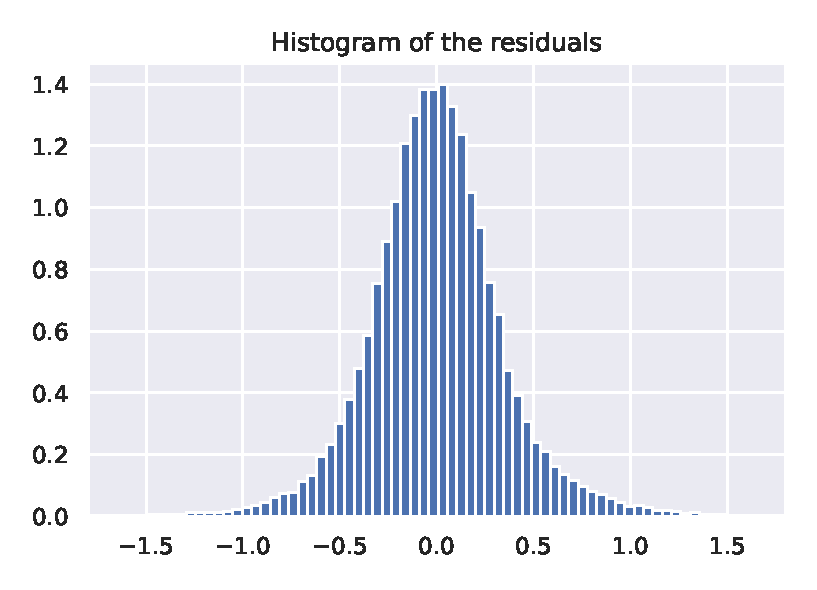
\includegraphics[width=0.45\textwidth]{histogram_residuals_slr.eps}
    \caption{Histogram of the residuals of simple linear regression model.}
    \label{fig:histogram-residuals-slr}
\end{figure}

\begin{figure*}
    \centering
    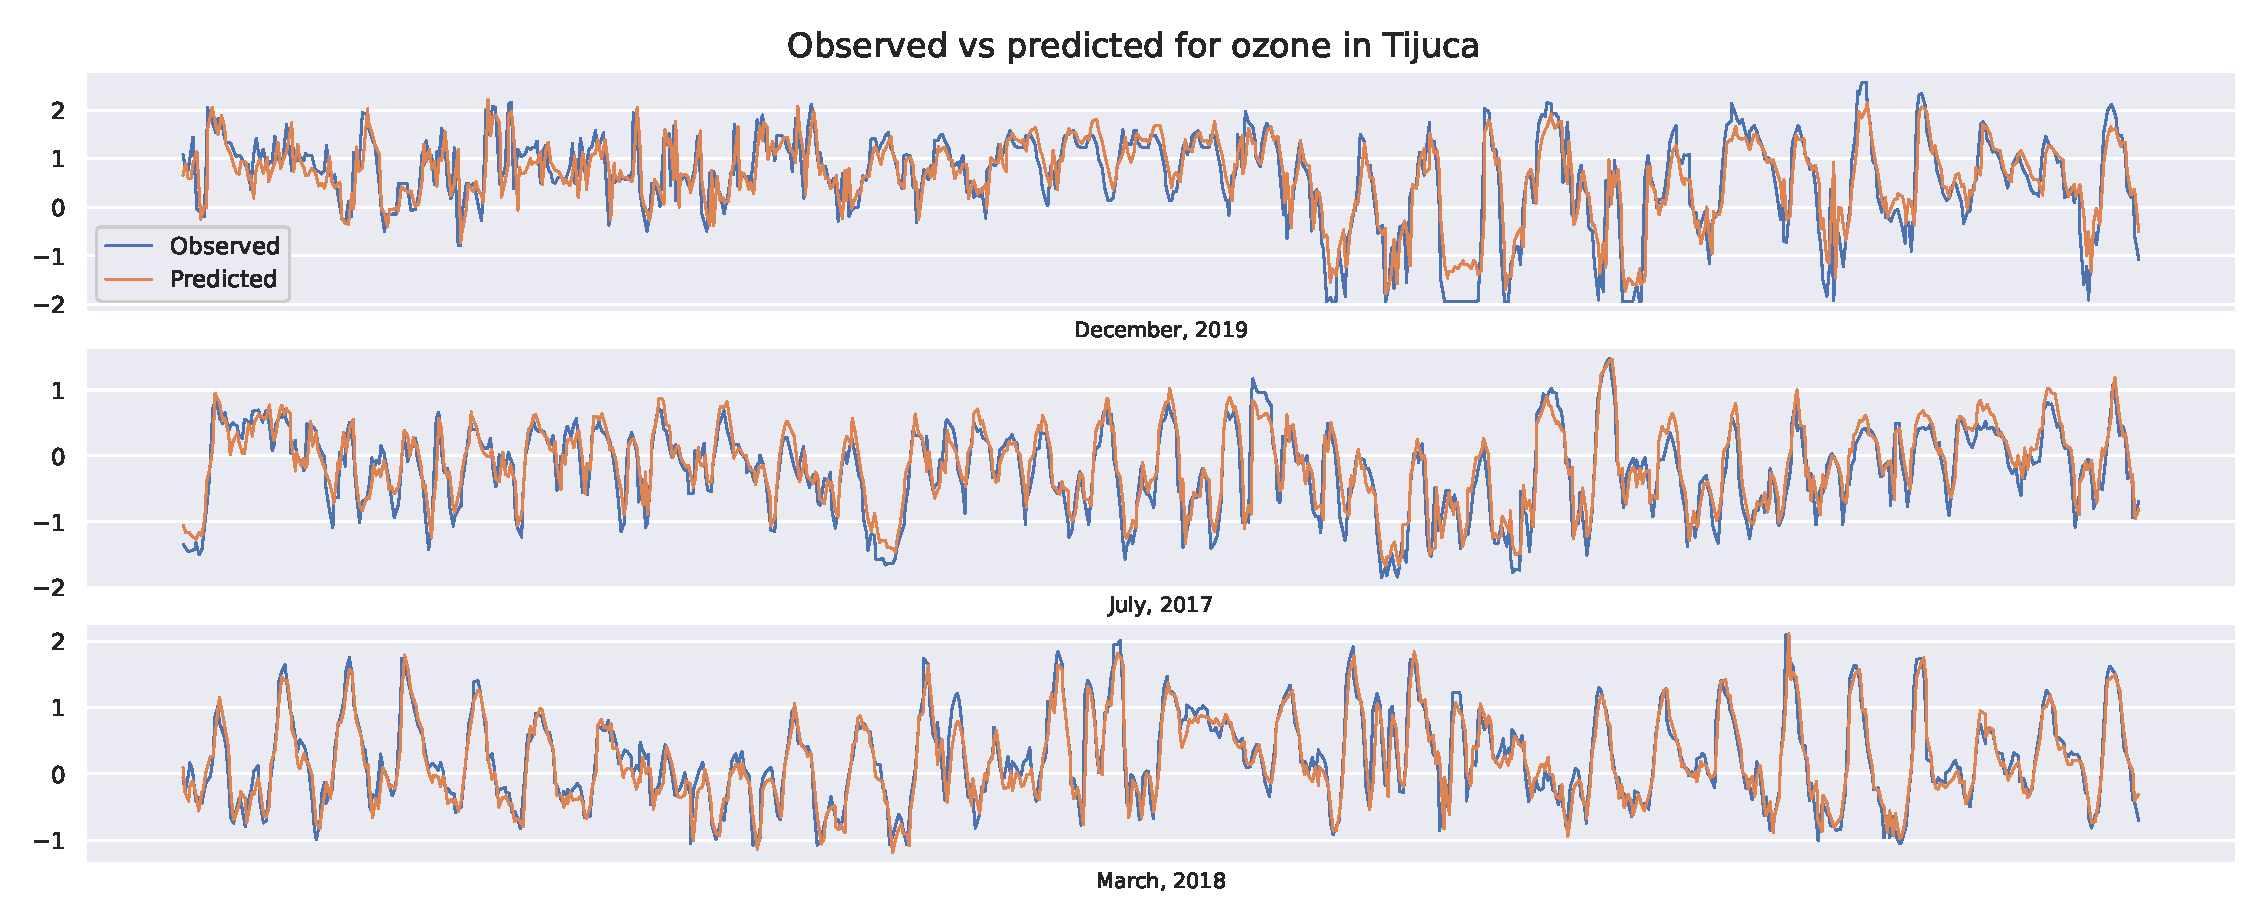
\includegraphics[width=\textwidth]{observed-fitting-ozone-tijuca.eps}
    \caption{Observed and predicted ozone values for different months in Tijuca.}
    \label{fig:observed-fitting-ozone-tijuca}
\end{figure*}

\subsubsection{PM\texorpdfstring{$_{10}$}{10}}

\subsubsection{AIQ}

\subsection{Aggregated results}

\subsubsection{CO}

\subsubsection{O\texorpdfstring{$_3$}{3}}

\subsubsection{PM\texorpdfstring{$_{10}$}{10}}

\subsubsection{AIQ}

\subsection{Model for other locations}

Here, we want to make predictions about pollutant levels at other not measured
sites. Given that each location has a specific model, the prediction
is the weighted mean regarding each prediction 



\begin{enumerate}
    \item 1 modelo para cada gás e cada estação. 
    \item Temos 7 opções de modelos até o momento (analisando friamente, 23 x
    7 = 161 modelos a serem fittados e analisados). 
    \item Como realizar tantos experimentos para cada modelo de forma
    automática? \com{A ideia é escrever um código para escolha de hiperparâmetros e
    reporte de resultados automaticamente.}
    \item Pegar uma estação para analisar os resultados mais cuidadosamente. 
    \item Testes de significância.  
\end{enumerate}

Lembrar de 

\begin{enumerate}
    \item Testar estacionaridade de cada série; 
    \item Lembrar de inverter os dados pelo power transformation: ler p2, fazer power transform. 
\end{enumerate}



\section{Discussion and Future work}
\label{sec:discussion}


\section{Conclusion}
\label{sec:conclusion}


\newpage

%\appendix

%\newpage

\bibliography{sections/biblio} 

\end{document}